La siguiente pirámide cuadrangular tiene base con lados de 12 unidades de longitud.
La altura vertical de la pirámide es 15 unidades, como se muestra en la figura \ref{fig:pitagoras3D_piram_03}:\\
\begin{figure}[H]
    \begin{center}
        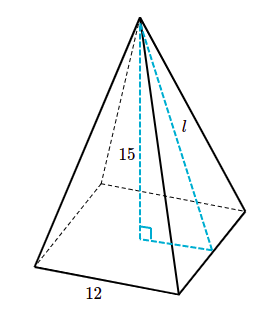
\includegraphics[width=0.4\textwidth]{../images/pitagoras3D_piram_03.png}
    \end{center}
    \caption{}
    \label{fig:pitagoras3D_piram_03}
\end{figure}
\textbf{¿Cuál es la longitud de $l$ (la altura de una de las caras triangulares)?}\\
\textit{Redondea tu respuesta a la décima más cercana.}
